Das Spiel Kuromasu (von japanisch
\begin{CJK}{UTF8}{min}黒枡マスはどこだ\end{CJK}, Kuromasu wa doko da,
``wo sind die schwarzen Felder?'')
wird auf einem $m\times n$-Spielfeld gespielt, in dem einzelne Felder
mit einer Zahl versehen sind.
Die Aufgabe des Spielers ist, einzelne Felder schwarz zu färben,
dabei aber folgende Regeln einzuhalten:
\begin{enumerate}
\item
Felder mit einer Zahl müssen weiss bleiben.
\item
Schwarze Felder dürfen nicht horizontal oder vertikal benachbart sein.
\item
Alle weissen Felder müssen horizontal oder vertikal miteinander
verbunden sein.
\item
Von einem Feld mit einer Zahl aus sind genau so viele weisse Felder
sichtbar, wie die Zahl angibt.
Ein Feld $B$, welches in der gleichen Zeile oder Spalte liegt wie das Feld $A$,
gilt als von $A$ aus sichtbar, wenn keine schwarzen Felder
zwischen $A$ und $B$ liegen.
\end{enumerate}
Die Abbildung zeigt links ein Kuromasu-Rätsel.
Im Feld rechts ist die Lösung eingezeichnet.
Die 11 hellrot hinterlegten Felder in der 6.~Zeile und in der 7.~Spalte
sind vom Feld mit der Zahl 11 aus sichtbar.
\begin{center}
\def\punkt#1#2{ ({0.6*(#1)},{0.6*(#2)}) }
\def\zahl#1#2#3{
	\draw \punkt{#1+0.5}{#2+0.5} circle[radius=0.28];
	\node at \punkt{#1+0.5}{#2+0.46} {$#3\mathstrut$};
}
\def\zahlen{
	\zahl{0}{2}{7}
	\zahl{0}{7}{9}
	\zahl{1}{6}{10}
	\zahl{2}{0}{2}
	\zahl{2}{1}{7}
	\zahl{2}{5}{12}
	\zahl{2}{10}{9}
	\zahl{4}{5}{8}
	\zahl{4}{8}{12}
	\zahl{6}{2}{2}
	\zahl{6}{5}{11}
	\zahl{8}{0}{5}
	\zahl{8}{5}{3}
	\zahl{8}{9}{7}
	\zahl{8}{10}{8}
	\zahl{9}{4}{3}
	\zahl{10}{3}{3}
	\zahl{10}{8}{16}
}
\def\schwarz#1#2{
	\fill[color=gray!60] \punkt{#1}{#2} rectangle \punkt{#1+1}{#2+1};
}
\def\feld{
	\draw \punkt{0}{0} rectangle \punkt{11}{11};
	\foreach \i in {1,...,10}{
		\draw \punkt{\i}{0} -- \punkt{\i}{11};
		\draw \punkt{0}{\i} -- \punkt{11}{\i};
	}
	\zahlen
}
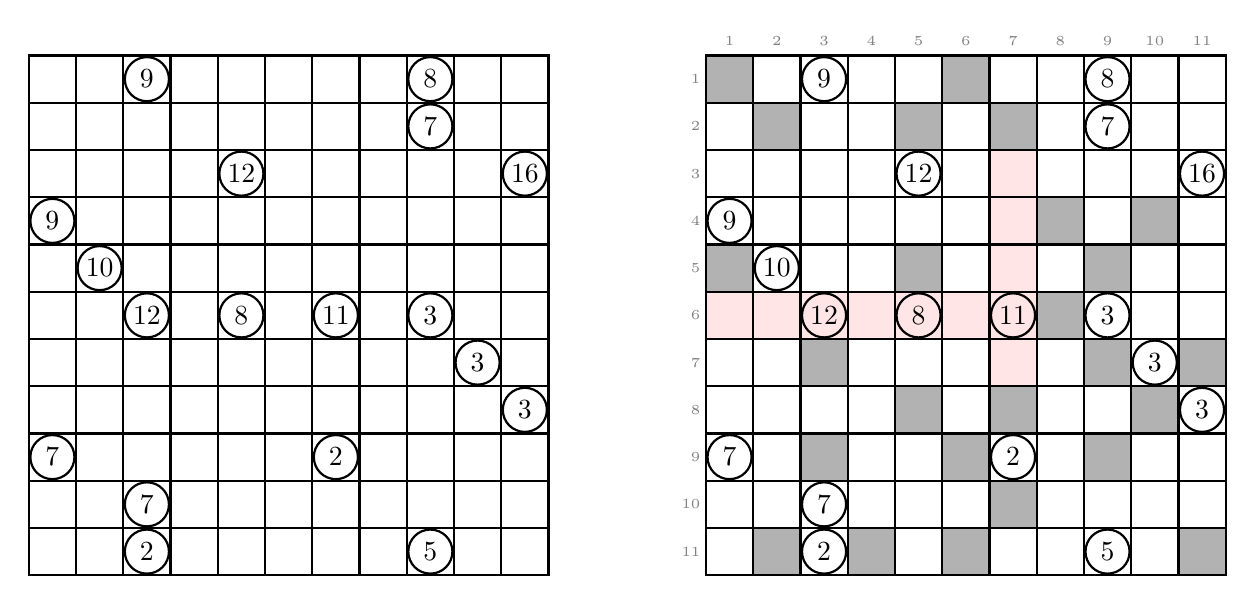
\begin{tikzpicture}[>=latex,thick]
\begin{scope}[xshift=-4.3cm]
\feld
\end{scope}
\begin{scope}[xshift=4.3cm]
\fill[color=red!10]
	\punkt{0}{5}
	-- \punkt{6}{5}
	-- \punkt{6}{4}
	-- \punkt{7}{4}
	-- \punkt{7}{9}
	-- \punkt{6}{9}
	-- \punkt{6}{6}
	-- \punkt{0}{6}
	-- cycle;
\schwarz{0}{6}
\schwarz{0}{10}
\schwarz{1}{0}
\schwarz{1}{9}
\schwarz{2}{2}
\schwarz{2}{4}
\schwarz{3}{0}
\schwarz{4}{3}
\schwarz{4}{6}
\schwarz{4}{9}
\schwarz{5}{0}
\schwarz{5}{2}
\schwarz{5}{10}
\schwarz{6}{1}
\schwarz{6}{3}
\schwarz{6}{9}
\schwarz{7}{5}
\schwarz{7}{7}
\schwarz{8}{2}
\schwarz{8}{4}
\schwarz{8}{6}
\schwarz{9}{3}
\schwarz{9}{7}
\schwarz{10}{0}
\schwarz{10}{4}
\feld
\foreach \x in {1,...,11}{
	\node[color=gray] at \punkt{\x-0.5}{11.3} {\tiny \x};
}
\foreach \y in {1,...,11}{
	\node[color=gray] at \punkt{0.1}{11.5-\y} [left] {\tiny \y};
}
\end{scope}
\end{tikzpicture}
\end{center}
Kann eine nichtdeterministische Turing-Maschine in polynomieller Zeit
entscheiden, ob ein Ku\-ro\-ma\-su-Rätsel eine Lösung hat?

\begin{loesung}
Die Frage ist gleichbedeutend damit, dass Kuromasu in der Klasse
NP ist.
Kuromasu ist sicher entscheidbar, da man alle $2^{nm}$ Einfärbungen
des Spielfeldes durchprobieren kann.
Es ist in NP genau dann, wenn es einen polynomiellen Verifizierer 
dafür gibt.

Als Lösungszertifikat werden die schwarzen Felder verlangt.
Dafür werden die folgenden Verifikationsschritte durchgeführt:
\begin{center}
\begin{tabular}{|c|p{12cm}|>{$}c<{$}|}
\hline
Schritt&Verifikation\strut&\text{Aufwand}\mathstrut\\
\hline
1&
Für jedes Feld mit einer Zahl überprüfe, ob es weiss ist.
&O(nm)\\
2&
Für jedes schwarz Feld überprüfe, ob die vertikalen und horizontalen
Nachbarn weiss sind
&O(nm)\\
3&
Ausgehend vom ersten weissen Feld, färbe alle horizontal oder vertikal
benachbarten weissen oder roten Felder rot ein, bis kein weiteren
Felder eingefärbt werden können.
Wenn ein weisse Feld übrig bleibt, ist die Regel 3 verletzt.
&O(n^2m^2)\\
4&
Von jedem Feld mit einer Zahl ausgehend zähle die horizontal und vertikal
benachbarten sichtbaren weissen Felder und überprüfe, ob die Anzahl
mit der Zahl übereinstimmt.
&O(n^2m+nm^2)\\
\hline
&Total\strut&O(n^2m^2)\mathstrut\\
\hline
\end{tabular}
\end{center}
Der Gesamtaufwand ist polynomiell, es gibt also einen polynomiellen
Verifizierer.
Damit ist gezeigt, dass Kuromasu in NP liegt.
\end{loesung}

\begin{diskussion}
Kuromasu wurde 1991 von Nikoli publiziert.
Jonas Kölker hat mit einer polynomiellen Reduktion von \textit{SAT}
gezeigt, dass Kuromasu NP-vollständig ist:
{\em Kurodoko is NP-complete}, Journal of Information Processing,
{\bf 20} (3), 694--706, \url{https://doi.org/10.2197/ipsjjip.20.694}.
\end{diskussion}


\begin{bewertung}
Entscheidbarkeit ({\bf E}) 1 Punkt,
Prinzip Verifizierer ({\bf V}) 1 Punkt,
Zertifikat spezifiziert ({\bf Z}) 1 Punkt,
Laufzeitschätzung ({\bf L}) 2 Punkte,
Schlussfolgerung polynomieller Verifizierer ({\bf S}) 1 Punkt.
\end{bewertung}

